\documentclass[a4paper,11pt]{article}
\usepackage[utf8]{inputenc}\usepackage[T1]{fontenc}
\usepackage[english]{babel}\usepackage{lmodern}\usepackage{microtype}
\usepackage{amsmath,amssymb}\usepackage{geometry}
\geometry{a4paper,left=2.2cm,right=2.2cm,top=2.0cm,bottom=2.0cm}
\usepackage{booktabs,array}\usepackage{xcolor}
\definecolor{bokug}{RGB}{0,135,60}\usepackage{tikz}
\usetikzlibrary{arrows.meta,calc}
\usepackage{fancyhdr}\pagestyle{fancy}
\renewcommand{\headrulewidth}{0.4pt}
\usepackage{enumitem}\setlength{\parindent}{0pt}\setlength{\parskip}{4pt}

\begin{document}
\fancyhead[L]{\small VU Mechanik – LAWI 100515 (PI)}\fancyhead[R]{\small SS 2026}\fancyfoot[C]{\thepage}
\begin{center}{\large\bfseries\color{bokug}University of Natural Resources and Life Sciences, Vienna (BOKU)}\\[2pt]{\large\bfseries VU Mechanik – LAWI 100515 (PI)}\\[4pt]Exam \textbf{Group A} \hfill Date: 26.06.2026\\[2pt]\rule{\linewidth}{0.4pt}\end{center}

\textbf{Given system}\par The planar system consists of bending beams and a truss connected by hinges.
\begin{center}
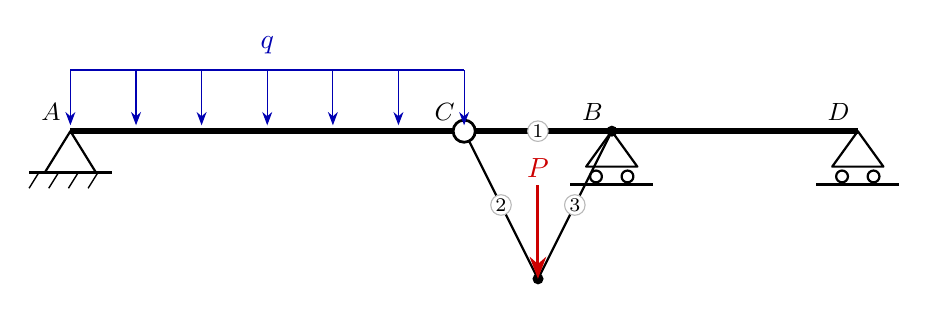
\begin{tikzpicture}[scale=1.250,>=Stealth,line join=round]
  \coordinate (P0) at (0.000,0.000);
  \coordinate (P1) at (4.000,0.000);
  \coordinate (P2) at (8.000,0.000);
  \coordinate (TO1) at (5.500,0.000);
  \coordinate (TU0) at (4.750,-1.500);
  \draw[thick] (P1) -- (TO1);
  \draw[thick] (P1) -- (TU0);
  \draw[thick] (TU0) -- (TO1);
  \draw[line width=2.2pt] (P0) -- (P1);
  \draw[line width=2.2pt] (P1) -- (P2);
  \fill (P1) circle (1.6pt);
  \fill (TO1) circle (1.6pt);
  \fill (TU0) circle (1.6pt);
  \draw[fill=white,line width=1pt] (P1) circle (3.2pt);
  \draw[thick] (0.000,0.000) -- (-0.260,-0.420) -- (0.260,-0.420) -- cycle;
  \draw[line width=1pt] (-0.420,-0.420) -- (0.420,-0.420);
  \draw[line width=0.5pt] (-0.320,-0.420) -- (-0.420,-0.580);
  \draw[line width=0.5pt] (-0.120,-0.420) -- (-0.220,-0.580);
  \draw[line width=0.5pt] (0.080,-0.420) -- (-0.020,-0.580);
  \draw[line width=0.5pt] (0.280,-0.420) -- (0.180,-0.580);
  \draw[thick] (8.000,0.000) -- (7.740,-0.360) -- (8.260,-0.360) -- cycle;
  \draw[thick] (7.840,-0.460) circle (0.06) (8.160,-0.460) circle (0.06);
  \draw[line width=1pt] (7.580,-0.540) -- (8.420,-0.540);
  \draw[thick] (5.500,0.000) -- (5.240,-0.360) -- (5.760,-0.360) -- cycle;
  \draw[thick] (5.340,-0.460) circle (0.06) (5.660,-0.460) circle (0.06);
  \draw[line width=1pt] (5.080,-0.540) -- (5.920,-0.540);
  \node[circle,fill=white,draw=gray!55,inner sep=0.5pt,font=\scriptsize] at (4.750,0.000) {1};
  \node[circle,fill=white,draw=gray!55,inner sep=0.5pt,font=\scriptsize] at (4.375,-0.750) {2};
  \node[circle,fill=white,draw=gray!55,inner sep=0.5pt,font=\scriptsize] at (5.125,-0.750) {3};
  \draw[->,blue!70!black] (0.000,0.620) -- (0.000,0.060);
  \draw[->,blue!70!black] (0.667,0.620) -- (0.667,0.060);
  \draw[->,blue!70!black] (1.333,0.620) -- (1.333,0.060);
  \draw[->,blue!70!black] (2.000,0.620) -- (2.000,0.060);
  \draw[->,blue!70!black] (2.667,0.620) -- (2.667,0.060);
  \draw[->,blue!70!black] (3.333,0.620) -- (3.333,0.060);
  \draw[->,blue!70!black] (4.000,0.620) -- (4.000,0.060);
  \draw[blue!70!black,thick] (0.000,0.620) -- (4.000,0.620);
  \node[blue!70!black] at (2.000,0.870) {$q$};
  \draw[->,red!80!black,line width=1.1pt] (4.750,-0.550) -- (4.750,-1.500);
  \node[red!80!black] at (4.750,-0.370) {$P$};
  \node[font=\small] at (0.000,0.000) [xshift=-7pt,yshift=7pt] {$A$};
  \node[font=\small] at (4.000,0.000) [xshift=-7pt,yshift=7pt] {$C$};
  \node[font=\small] at (8.000,0.000) [xshift=-7pt,yshift=7pt] {$D$};
  \node[font=\small] at (5.500,0.000) [xshift=-7pt,yshift=7pt] {$B$};
\end{tikzpicture}
\end{center}
\textbf{Given quantities:}\quad $a=4$\,m\quad $\ell=1,5$\,m\quad $h=1,5$\,m\quad $q=5$\,kN/m\quad $P=12$\,kN
\par\medskip
\textbf{Tasks}\par
\begin{enumerate}[label=\textbf{\arabic*.}]
  \item Determine the degree of static determinacy.
  \item Compute all support reactions and hinge forces.
  \item Determine all truss member forces (tension/compression).
  \item Draw the section forces $N$, $V$, $M$ of the bending beams.
\end{enumerate}
\end{document}